\documentclass{beamer}
\usepackage{lmodern}
\usepackage{HECbeamer} 
% \usepackage{pgfpages}
% \pgfpagesuselayout{4 on 1}[letterpaper, landscape, border shrink=5mm]
\title[\color{white}{MATH60604A Likelihood-based inference}]{\texorpdfstring{MATH60604A \\Statistical modelling \\ \S 3 - Likelihood-based inference}{MATH60604A \\Statistical modelling \\ \S~3 - Likelihood-based inference}}
\author{}
\institute{HEC Montréal\\
Department of Decision Sciences}
\date{} 
% \newcommand{\AIC}{\ensuremath{\mathsf{AIC}}}
% \newcommand{\BIC}{\ensuremath{\mathsf{BIC}}}
\begin{document}
\frame{\titlepage}
% 
% \begin{frame}[fragile]
% \frametitle{Chapter overview}
% 
% 
% \begin{tcolorbox}[colback=white, colframe=hecblue, title= Likelihood methods]
% \vp\vp
% \tableofcontents
% 
% \end{tcolorbox}
% \end{frame}
\section{Likelihood function}
\begin{frame}
\frametitle{Likelihood}
\bi

\item The \alert{likelihood} $L(\bs{\theta})$ is a function of the \textbf{parameters} of the distribution, say $\bs{\theta}$.

\bi \item The likelihood  gives the probability of observing a sample under a postulated distribution whose parameters are $\bs{\theta}$.
\item The likelihood treats the observations as fixed.
\ei

\item The \alert{maximum likelihood} estimator $\hat{\bs{\theta}}$ is the value of $\bs{\theta}$ that maximizes the likelihood.
\bi \item the value that makes the observed sample the most \alert{likely} or \alert{plausible}. 
\item scientific thinking: whatever we observe, we have expected to observe.
\ei
\ei
\end{frame}
\begin{frame}
\frametitle{Bernoulli trials}
\bi
\item Suppose we want to estimate the probability that an event occurs, which we assume is constant.
\item For example, whether a customer buys a product or not, whether a study participant completes a task or not, etc.
\item We have a sample size of $n$ with $X_i$ assumed to come from a Bernoulli distribution with probability $p$, meaning 
\begin{align*}
\P{X_i=1}&=p, \qquad \P{X_i=0}=1-p.                                 
\end{align*}

\item By convention, ``$1$'' denotes a success and ``$0$'' a failure.
\ei
\end{frame}

\begin{frame}[fragile]
\frametitle{Joint probability of outcomes in Bernoulli example}
 A compact way of writing the mass function is
\begin{align*}
\P{X_i=x_i  \mid p}=p^{x_i} (1-p)^{1-x_i}, \qquad x_i \in \{0, 1\}.
\end{align*}
Since the observations are independent, the joint probability of a given result is the product of the probabilities for each observation,
\begin{align*}
\P{X_1=x_1, \ldots, X_n=x_n \mid p}&=\prod_{i=1}^n \P{X_i=x_i  \mid p}
\\&=\prod_{i=1}^n  p^{x_i} (1-p)^{1-x_i}.
\end{align*}
\end{frame}


\begin{frame}[fragile]
\frametitle{Likelihood of the Bernoulli model}
The likelihood for the random sample is 
\begin{align*}
L(p; \bs{X}) &=\prod_{i=1}^n p^{X_i} (1-p)^{(1-X_i)}\\&= p^{\Sigma_{i=1}^n X_i}(1-p)^{n-\Sigma_{i=1}^n X_i}.
\end{align*}
% \item The \textbf{likelihood function} is a function of the parameters, treating the observations as fixed.
% \item For a given value of $p$ and fixed $\bs{x}$, $L(p)$ is the \alert{probability of observing this sample}. 
% \item The maximum likelihood estimator of $p$ is \alert{the value of $p$ that maximizes the likelihood function} $L(p; \bs{X})$. 
% \bi \item the value that makes the observed sample the most \alert{likely} or \alert{plausible}. 
% \item scientific reasoning: whatever we observe, we expected to observe.\ei
% \ei
% \end{frame}
% 
% \begin{frame}[fragile]
% \frametitle{Numerical example}
% \bi 
This likelihood is (up to normalizing constant) the same as that of a binomial sample of size $n$ with probability of success $p$.
\bi
\item the likelihood only depends on the number of successes, regardless of the ordering.
\ei
 Suppose that we have $n=10$ observations, eight of which are successes.
 \bi
\item The likelihood is $L(p)=p^8(1-p)^2$. %and the maximum likelihood estimate $\widehat{p}$ is $0.8$.
\ei
\end{frame}

 \begin{frame}[fragile]
\frametitle{Plot of the likelihood function $L(p)$}

\begin{center}
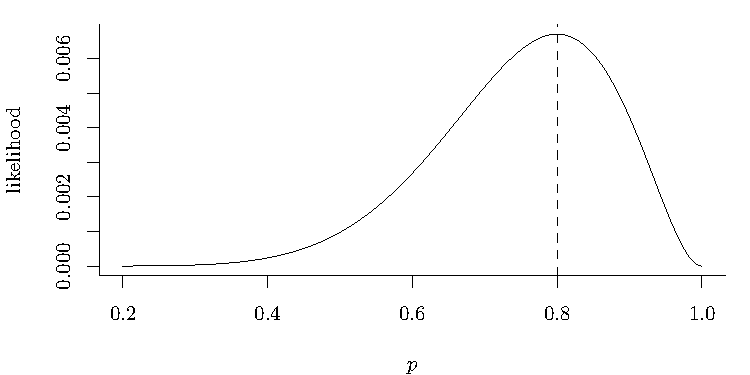
\includegraphics[width = \linewidth]{img/c3/05-likelihood.pdf}
\end{center}
\end{frame}
\begin{frame}
\frametitle{Log-likelihood for Bernoulli sample}
\bi
\item The log-likelihood function is
\begin{align*}
\ell(p)=\sum_{i=1}^n \ln\left\{p^{x_i}(1-p)^{1-xi}\right\}
\end{align*}
\item Using the property $\ln(a^b)=b\ln(a)$, rewrite
\begin{align*}
\ell(p)=\ln(p)\sum_{i=1}^n x_i + \ln(1-p) \left(n-\sum_{i=1}^n x_i\right).
\end{align*}
\item In our numerical example, with eight ones and two zeros, the log-likelihood is $\ell(p)=8 \ln(p) + 2 \ln(1-p)$.
\ei
\end{frame}

% 
% \begin{frame}
% \frametitle{Log-likelihood}
% \bi
% \item Maximization of the likelihood is sometimes numerically unstable, since we deal with a \textbf{product} of small numbers between zero and one.
% \item Since logarithm is a strictly increasing function, maximizing the natural logarithm $\ln \equiv \ln$ of the likelihood is equivalent to maximizing the likelihood.
% \bi 
% \item The log of a product is equal to the sum of logs, that is, 
% $\ln(ab) =\ln(a) +\ln(b)$, so the product over $n$ terms becomes a sum.
% \item It is usually easier to work with sums rather than products. 
% \ei 
%  \item We call the function $\ell(\bs{\theta}) = \ln\{L(\bs{\theta})\}$ the \alert{\textbf{log-likelihood}} function.
% \ei
% \end{frame}

\begin{frame}
\frametitle{Plot of the log-likelihood function $\ell(p)$}

\begin{center}
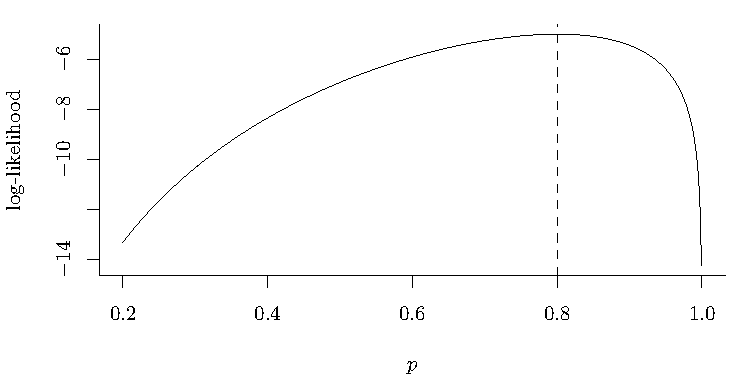
\includegraphics[width = \linewidth]{img/c3/05-loglikelihood.pdf}
\end{center}
% It's a little less clear this time, but the maximum is still achieved at the value $p=0.8$ for this sample.
\end{frame}

\begin{frame}
\frametitle{Maximum likelihood estimator}
Differentiating $\ell(p)$ with respect to $p$,
\begin{align*}
\frac{\mathrm{d}}{\mathrm{d}p} \ell(p)=\frac{1}{p} \sum_{i=1}^n x_i-\frac{1}{(1-p)}\left(n-\sum_{i=1}^n x_i \right).
\end{align*}
Solving the score equation $U(p)=\d \ell(p)/\d p
 =0$, we find
\begin{align*}
\widehat{p}=\frac{1}{n} \sum_{i=1}^n x_i = \overline{x}.
\end{align*}
The second derivative,
\begin{align*}
  \frac{\d^2 \ell(p)}{\d p^2} &= -\frac{1}{p^2} \sum_{i=1}^n x_i-\frac{1}{(1-p)^2}\left(n-\sum_{i=1}^n x_i \right),   
\end{align*}
is negative, so $L(p)$ thus achieves a maximum at $\widehat{p}$ and the maximum likelihood estimator of $p$ is the sample \textbf{proportion of ones}.
\end{frame}

\begin{frame}
 \frametitle{Information}
 The observed information $j(p) = - \d^2 \ell(p)/\d p^2$ and 
 \begin{align*}
j(\widehat{p}) &= \frac{n}{\overline{x}} + \frac{n}{(1-\overline{x})} = \frac{n}{\overline{x}(1-\overline{x})}  
\end{align*}
so, the estimated variance of $\widehat{p}$ is $j^{-1}(\widehat{p}) = 0.016$ and the standard error $0.1265$.

The Fisher information is 
\[
i(\theta) = \frac{n}{p(1-p)}.
\]
\bi \item For independent and identically distributed data, the total information in the sample is $n$ times that of an individual observation (information accumulates linearly).
\ei
\end{frame}

\begin{frame}
 \frametitle{Testing procedure}
 Suppose we are interested in the two-sided hypothesis 
 \[\Hy_0: p_0 = 0.5 \qquad \text{ versus } \qquad \Hy_a: p_0 \neq 0.5.\]
 
 The three likelihood-based tests for this hypothesis are:
 \bi \item 
 the Wald test 
  \[W(p_0) = \frac{(\widehat{p} - p_0)^2}{\Va{\widehat{p}}} = \frac{(\widehat{p}-p_0)^2}{\widehat{p}(1-\widehat{p})/n}\]
  \item  the score test 
  \[S(p_0) = \frac{U^2(p_0)}{i(p_0)} = \frac{(\widehat{p}-p_0)^2}{p_0(1-p_0)/n}\]
 \item the likelihood ratio test
 \begin{align*}
  R(p_0) &= 2\{\ell(\widehat{p}) - \ell(p_0)\} 
  \\&= 2 \left\{ y\ln \pfrac{\widehat{p}}{p_0} + (n-y)\ln\pfrac{1-\widehat{p}}{1-p_0}\right\}
 \end{align*}
\ei
 \end{frame}
  \begin{frame}
 \frametitle{Illustration of likelihood-based tests}
 \begin{center}
  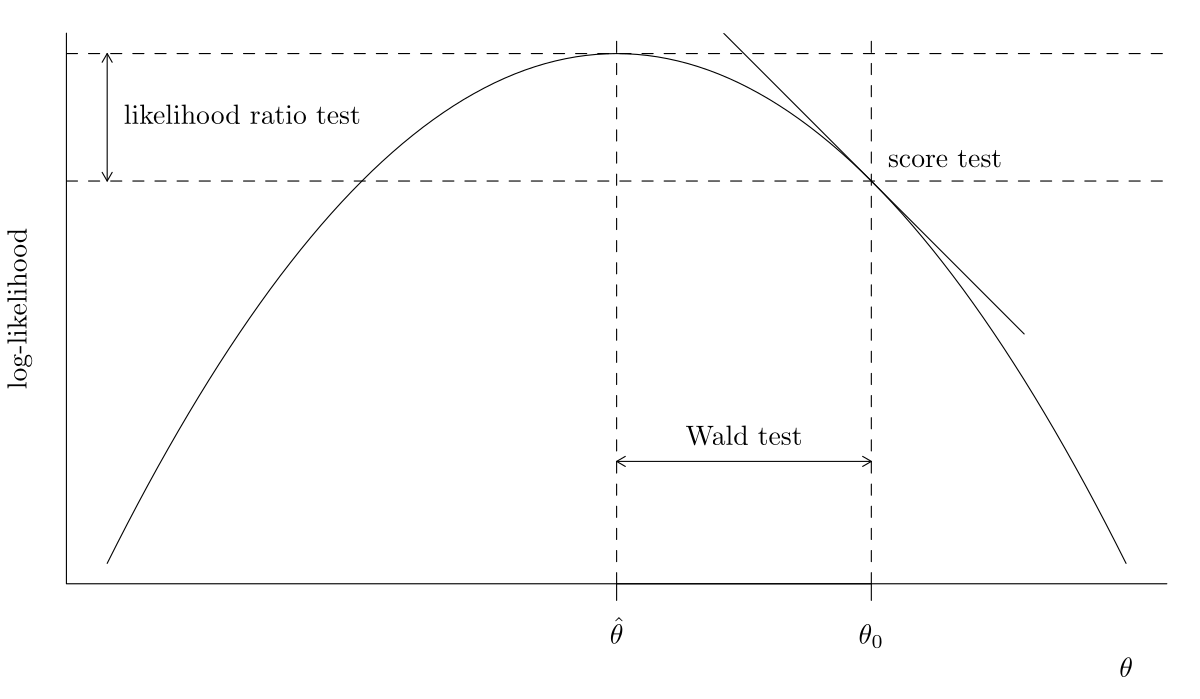
\includegraphics[width = \linewidth]{img/c3/likelihood_tests}
 \end{center}
\end{frame}
 \begin{frame}[fragile]
 \frametitle{Numerical results and confidence intervals}
 \bi 
 \item With 8 successes out of 10 trials, the statistics equal $W=5.62$, $S=3.6$, $R = 3.855$;
 \item we compare these values with the $0.95$ quantile of the $\chi^2_1$ distribution, $3.84$.
 \ei
 \bi \item 
In small sample size or when the sampling distribution is strongly asymmetric, the Wald test is \alert{unreliable}.
\item 
 Inverting the Wald statistic gives a 95\% confidence interval \[\widehat{p} \pm \mathfrak{z}_{1-\alpha/2}\sqrt{\frac{\widehat{p}(1-\widehat{p})}{n}}\]
 \item The 95\% Wald-based confidence interval is $0.8 \pm 1.96 \cdot 0.1265 = [0.55, 1.048]$!
 \item Compare with the 95\% confidence intervals based on
 \bi \item the likelihood ratio statistic, $[0.5005, 0.964]$.
 \item the score statistic, $[0.49, 0.943]$.
  \ei 
  \ei 
  {\footnotesize Solve $\{p: S(p) \leq 3.84\}$ and $\{p: R(p) \leq 3.84\}$ via root finding.}
\end{frame}


% \begin{frame}
% \frametitle{General definition of likelihood}
% \bi
% \item In the preceding example, there was only one parameter ($p$).
% \item Most of the time, the model contains a large number of parameters. 
% 
% \ei
% \end{frame}
% \begin{frame}
% \frametitle{Estimating the mean and variance of a normal sample}
% % 
% % Illustration: \textbf{Understanding Maximum Likelihood} by Kristoffer Magnusson, \url{https://rpsychologist.com/d3/likelihood/}
% 
% \bi
% \item Suppose we have an independent normal sample of  size $n$ with mean $\mu$ and variance $\sigma^2$, where
% \begin{align*}
% X_i \simiid \mathcal{N}(\mu, \sigma^2).
% \end{align*}
% \item The vector of parameters is $\bs{\theta}=(\mu, \sigma^2)$. 
% \item Recall that the density of the normal distribution is
% 
% \begin{align*}
% f(x \mid \bs{\theta})=\frac{1}{(2\pi \sigma^2)^{1/2}}\exp\left\{-\frac{1}{2\sigma^2}(x-\mu)^2\right\}, \qquad x \in \R.
% \end{align*}
% \ei
% \end{frame}
% 
% \begin{frame}
% \frametitle{Example : estimating the mean and variance of a normally-distributed population}
% \bi
% \item For a sample $\bs{X}=\bs{x}$, the likelihood is 
% \begin{align*}
% L(\bs{\theta})=&\prod_{i=1}^n\frac{1}{({2\pi \sigma^2})^{1/2}}\exp\left\{-\frac{1}{2\sigma^2}(x_i-\mu)^2\right\}\\
% =&(2\pi \sigma^2)^{-n/2}\exp\left\{-\frac{1}{2\sigma^2}\sum_{i=1}^n(x_i-\mu)^2\right\}.
% \end{align*}
% \item The log-likelihood is
% \begin{align*}
% \ell(\bs{\theta})=-\frac{n}{2}\ln(2\pi) -\frac{n}{2}\ln(\sigma^2)-\frac{1}{2\sigma^2}\sum_{i=1}^n (x_i-\mu)^2.
% \end{align*}
% % \item This is a function of two variables, $\mu$ and $\sigma^2$. \alert{The ML estimators are obtained by finding the values of $\mu$ and $\sigma^2$ that maximize this function.}
% \ei
% \end{frame}
% 
% \begin{frame}
% \frametitle{Analytic expression for MLE of normal sample}
% This is another example for which we're able to find the maximum likelihood estimator analytically. The \alert{score equations} are
% \begin{align*}
% \frac{\partial}{\partial \mu} \ell(\bs{\theta})=0 , \qquad \frac{\partial}{\partial \sigma^2} \ell(\bs{\theta})=0.
% \end{align*}
% One can show that 
% \begin{align*}
% \hat{\mu}=\overline{X}=\frac{1}{n} \sum_{i=1}^n X_i, \qquad \hat{\sigma}^2=\frac{1}{n}\sum_{i=1}^n (X_i-\overline{X})^2,
% \end{align*}
% are the maximum likelihood estimators for the two parameters.
% 
% \end{frame}
% 
% \begin{frame}
% \frametitle{Estimating the mean and variance of a normal distribution}
% \bi
% \item Intuitively, we would expect the estimator of the theoretical mean $\mu$ to just be the sample mean. 
% \item However, the estimator of $\sigma^2$ is not the sample variance estimator,
% \begin{align*}
% S^2=\frac{1}{n-1} \sum_{i=1}^n (X_i-\overline{X})^2
% \end{align*}
% \item In one case we divide by $n$ (maximum likelihood estimator); in the other we divide by $(n -1)$. 
% \item The two estimators are \textbf{consistent}, i.e., the estimate will get arbitrarily close to the true value $\sigma^2$ as $n \to \infty$.
% \ei
% \end{frame}
% 
% \begin{frame}
% \frametitle{Unbiasedness}
% \bi
% \item An estimator of $\theta_i$ is \textbf{unbiased} if its expectation is equal to $\theta_i$.
% \bi \item On average, the estimate is centered at the true value, regardless of the sample size $n$.\ei
% \item The maximum likelihood estimator for the mean of a normal distribution is \alert{unbiased}, meaning that
% \begin{align*}
% \E{\hat{\mu}}=\mu
% \end{align*}
% \item One can show that $\E{S^2}=\sigma^2$ and so the sample variance estimator is unbiased.
% \item Since $\hat{\sigma}^2=(n-1)/n S^2$, it follows that the maximum likelihood estimator of $\sigma^2$ is \textbf{biased}. 
% \ei
% \end{frame}
% 
% 
% \begin{frame}
% \frametitle{Ordinary linear regression}
% Assuming normality of the errors,  the least square estimators of $\bs{\beta}$ coincide with the maximum likelihood estimator of $\bs{\beta}$.
% \bi \item 
% Recall the linear regression model, 
% \begin{align*}
% Y_i=\beta_0+\beta_1 \mathrm{X}_{i1}+\beta_2 \mathrm{X}_{i2}+\ldots +\beta_p \mathrm{X}_{ip} + \eps_i, \qquad  (i=1, \ldots, n),
% \end{align*}
% where the errors $ \eps_i\simiid \Cn(0, \sigma^2)$.
% \item The linear model has $p+2$ parameters: $\beta_0, \beta_1, \ldots, \beta_p $ and $ \sigma^2$. 
% \item The log-likelihood is 
% \begin{align*}
% \ell(\bs{\theta})&=-\frac{n}{2} \ln(2\pi)-\frac{n}{2} \ln (\sigma^2)\\& \quad -\frac{1}{2\sigma^2}\sum_{i=1}^n \left(Y_i-\beta_0-\sum_{j=1}^p \beta_j\mathrm{X}_{ij}\right)^2.
% \end{align*}
% \ei
% \end{frame}
% 
% 
% \begin{frame}
%  \frametitle{Least squares and maximum likelihood estimator}
% \bi
% \item Maximizing the log-likelihood with respect to $\beta_0, \ldots, \beta_p$ is equivalent to
% minimizing the sum of squared errors,
% \begin{align*}
% \sum_{i=1}^n \left(Y_i-\beta_0-\sum_{j=1}^p \beta_j\mathrm{X}_{ij}\right)^2.
% \end{align*}
% \item This objective function is the same as that of least squares.
% \item The least-square estimator $\hat{\bs{\beta}}$ of $\bs{\beta}$ is the maximum likelihood estimator.
% \ei
% \end{frame}
% 
% 
% 
% \begin{frame}
% \frametitle{Maximum likelihood estimator of the variance in linear regression}
% \bi
% \item The maximum likelihood estimator (MLE) of the variance $\sigma^2$ is
% \begin{align*}
% \hat{\sigma}^2=\frac{1}{n} \sum_{i=1}^n \left(Y_i-\hat{\beta}_0-\hat{\beta}_1\mathrm{X}_{i1}-\cdots-\hat{\beta}_p\mathrm{X}_{ip}\right)^2
% \end{align*}
% \item The usual estimator of  $\sigma^2$ is
% \begin{align*}
% S^2=\frac{\mathsf{SS}_e}{n -p-1},
% \end{align*}
% where $p+1$ is the number of $\beta$'s and $\mathsf{SS}_e $, the sum of squared residuals, is
% \begin{align*}
% \mathsf{SS}_e = \sum_{i=1}^n e_i^2= \sum_{i=1}^n \left(Y_i-\hat{\beta}_0-\hat{\beta}_1\mathrm{X}_{i1}-\cdots-\hat{\beta}_p\mathrm{X}_{ip}\right)^2.
% \end{align*} 
% \item $S^2$ is unbiased for $\sigma^2$, unlike $\hat{\sigma}^2$. Both estimators are consistent.
% \ei
% \end{frame}
% 
% \begin{frame}
% \frametitle{Linear regression}
% \bi
% \item The maximum likelihood estimator of the variance is biased, but this bias becomes negligible when the sample size increases and $n \gg p$.
% \item An alternative estimation method that tries to reduce the bias is \alert{residual maximum likelihood} (REML) or
% \alert{restricted maximum likelihood}). It uses the likelihood of a linear combination of the observations. 
% \item 
% This method is often preferable for mixed models (Chapter 7) and we recommend you use it. The method is also the default method for the \SASlang \texttt{proc mixed} procedure.
% \ei
% \end{frame}

% 
% \begin{frame}
% \frametitle{Properties of the maximum likelihood estimator (MLE)}
% 
% Several properties of maximum likelihood estimator makes it appealing for inference.
% \be
% \item The maximum likelihood estimator is \alert{\textbf{consistent}}, i.e., it converges to the correct value as the sample size increase (\textbf{asymptotically unbiased}).
% \item Under regularity conditions, the MLE is \alert{\textbf{asymptotically normal}}:
% \bi \item in large sample, the estimator is approximately normal;
% \item we use this to obtain the null distribution of classes of hypothesis tests and derive confidence intervals.
% \ei 
% \item The MLE are efficient, meaning they have the 
% \alert{smallest asymptotic mean squared error} (or the smallest asymptotic variance).
% 
% \ee
% \end{frame}
% 
% \begin{frame}
% \frametitle{Covariance estimates of parameters}
% The derivatives of the likelihood encode information about the model.
% \bi \item The score $S(\bs{\theta}) = \partial \ell(\bs{\theta}) / \partial \bs{\theta}$ is zero at the maximum likelihood estimator, meaning $S(\hat{\bs{\theta}})=\bs{0}$.
% \bi \item This can be used to check if our optimization routine found the MLE.
% \ei
% \item 
% The Hessian  $\mathbf{H}(\bs{\theta}) = \partial^2 \ell(\bs{\theta}) / \partial \bs{\theta} \partial \bs{\theta}^\top$ measures the curvature of the log-likelihood.
% % 
% % \item Under regularity conditions, the information matrix (i.e., the variance of the score) is \[\mathcal{I}(\hat{\bs{\theta}}) = -\E{\mathbf{H}(\bs{\theta})} = \Va{S(\bs{\theta})}.\]
% % \bi 
% % \item We can estimate the covariance matrix of $\hat{\bs{\theta}}$ by $\mathcal{I}^{-1}(\hat{\bs{\theta}})$.
% \item Often, we use the \textbf{observed information}, i.e., the negative of the inverse of the Hessian matrix evaluated at the MLE, $-\mathbf{H}^{-1}(\hat{\bs{\theta}})$, as estimate of the covariance matrix of the MLE.
% \bi \item The estimated \textbf{standard errors} of $\hat{\bs{\theta}}$  are the square root of the diagonal elements of $-\mathbf{H}^{-1}(\hat{\bs{\theta}})$.
% \ei
% \ei
% \end{frame}
% 
% \section{Likelihood tests}
% 
% \begin{frame}
%  \frametitle{Nested models and hypothesis tests}
%  \bi \item 
%  We consider a null hypothesis $\Hy_0$ that imposes restrictions on the possible values of $\bs{\theta}$ can take, relative to an unconstrained alternative $\Hy_1$. 
% \item We need two \textbf{nested} models: a ``full'' model, and a ``reduced'' model that is a subset of the full model where we impose $q$ restrictions. 
% \item The procedure involves fitting the two models and obtaining the maximum likelihood estimators of each of $\Hy_1$ and $\Hy_0$, respectively $\hat{\bs{\theta}}$ and $\hat{\bs{\theta}}_0$ for the parameters under $\Hy_0$.
% \ei 
% 
% 
% \vp\vp
%  {\footnotesize For example, the full model could be  a regression model with four predictor variables and the reduced model could include only the first 2 predictor variables, which is equivalent to setting $\Hy_0: \beta_3=\beta_4=0$.
%  
%  }
% \end{frame}
% \begin{frame}
% \frametitle{Likelihood-based tests}
% 
%  There are three classes of tests based on likelihood that can be used to compare \textbf{nested models}.
%  \bi \item likelihood ratio tests, which measure the drop in log-likelihood (\textbf{vertical distance}) from $\ell(\hat{\bs{\theta}})$ and $\ell(\hat{\bs{\theta}}_0)$.
%  \item Wald tests, which consider the standardized \textbf{horizontal distance} between $\hat{\bs{\theta}}$ and $\hat{\bs{\theta}}_0$.
%  \item score tests, which looks at the scaled gradient of $\ell$, evaluated \textbf{only}  at $\hat{\bs{\theta}}_0$ (\textbf{derivative} of $\ell$).
%  \ei
%   Asymptotically, all the tests are equivalent (in the sense that they lead to the same conclusions about $\Hy_0$).
%   
%   All of these test statistics follow asymptotically a $\chi^2_q$ distribution under $\Hy_0$ with $q$ restrictions.
%  
%  \end{frame}
% % Likelihood-based methods grant access to omnibus testing procedures.
% 
% % \bi
% % \item we measure deviation in terms of fit between the null model (under which restrictions are imposed on the possible values the parameters can take) and the alternative, for which the MLE is $\hat{\bs{\theta}}$.
% % \bi \item Let $\widehat{\bs{\theta}}_0$ denote the maximum likelihood estimator under $\Hy_0$ and $\hat{\bs{\theta}}$ under the alternative (no restriction).
% % \item By definition of MLE, $\ell(\widehat{\bs{\theta}}_0) \leq \ell(\widehat{\bs{\theta}})$.
% % \item We can also use the \textbf{gradient} of the log-likelihood, $S(\bs{\theta}) = \partial \ell(\bs{\theta}) / \partial \bs{\theta}$, the \textbf{score function}, to measure how far we are from the global optimum under $\Hy_0$, given that $S(\hat{\bs{\theta}})=\bs{0}$ under regularity conditions. 
% % \ei
% % \ei
% % \end{frame}
% 

% 
% 
% 
% % \begin{frame}
% % \frametitle{Likelihood ratio test}
% % \bi
% % 
% % \bi
% % \item The maximum log-likelihood value of the full model (unrestricted) is $\ell(\hat{\bs{\theta}})$.
% % \item The maximum log-likelihood value for the reduced model is $\ell(\hat{\bs{\theta}}_0)$
% % \ei
% % \item
% % \ei
% % \end{frame}
% 
% \begin{frame}
% \frametitle{Likelihood ratio test}
% The \textbf{likelihood ratio test statistic} is
% \begin{align*}
% D=2\{\ell(\hat{\bs{\theta}})-\ell(\hat{\bs{\theta}}_0)\}. 
% \end{align*}
% \bi 
% \item The null hypothesis $\Hy_0$ tested in this statistic is that the reduced model is an \textbf{adequate simplification} of the full model.
% \item If $\Hy_0$ is true,  $D \stackrel{\cdot}{\sim}\chi^2_q$, where the degrees of freedom $q$ are the number of restrictions. 
% \item The testing procedure is extremely general and has nice properties: invariance to reparametrization (unlike Wald tests), uniformly most powerful, etc.
% \bi 
% \item The $F$-test covered in linear regression is equivalent to the likelihood ratio test for the linear model
% \item but we used the exact distribution rather than the asymptotic one.
% \ei
% \ei
% \end{frame}
% 
% % 
% % \begin{frame}
% % \frametitle{Likelihood ratio test}
% % 
% % \bi
% % \item We just saw that the quantity $-2\ell(\hat{\bs{\theta}})$ is a measure of model fit  and can be used for selecting (via tests of restrictions) between \textbf{nested models}.
% % 
% %  \item The likelihood ratio test can \textbf{only} be used to compare \alert{nested models}.
% % % \item We can also use the quantity $-2\ell(\hat{\bs{\theta}})$ to construct powerful tests.  
% % \ei
% % \end{frame}
% 
% \begin{frame}
%  \frametitle{Score and Wald tests}
%  \textbf{Score tests}
%  \bi \item While rarely encountered, score tests use the score $S(\bs{\theta})$ of the full model, but only evaluated at $\hat{\bs{\theta}}_0$. They are often used when obtaining $\hat{\bs{\theta}}$ is costly or difficult.
% %  \item Specifically, the statistic takes the form
% %  \begin{align*}
% %   W_s = S(\hat{\bs{\theta}}_0)^\top \mathcal{I}^{-1}(\hat{\bs{\theta}}_0) S(\hat{\bs{\theta}}_0),
% %  \end{align*}
% %  where $S$ and $\mathcal{I}$ are the score and information under the \textbf{alternative hypothesis}.
% \ei 
% \textbf{Wald tests}
% \bi
%  \item The multivariate Wald test is 
%  \begin{align*}
%   W^2 = -(\hat{\bs{\theta}}-\hat{\bs{\theta}}_0)^\top \mathbf{H}^{-1}(\hat{\bs{\theta}})  (\hat{\bs{\theta}}-\hat{\bs{\theta}}_0).
%  \end{align*}
%  \item When $\theta$ is one-dimensional, the Wald statistic is often reported as $W = (\hat{\theta}-\theta_0)/\mathrm{se}(\hat{\theta})$, which is approximately $ \Cn(0,1)$ under $\Hy_0$.
% \ei
% \end{frame}
% \begin{frame}
%  \frametitle{Confidence intervals}
%  
%  \begin{center}
%   \includegraphics[width = \linewidth]{figures/05-likelihood_ci}
%  \end{center}
% 
% \end{frame}
% \begin{frame}
%  \frametitle{Properties of Wald-based confidence intervals}
% The Wald-based two-sided 95\% confidence interval for a single parameter  $\theta$ are of the form \[\hat{\theta} \pm q_{1-\alpha/2}\mathrm{se}(\hat{\theta}),\] where $q_{1-\alpha/2}$ is the $1-\alpha/2$ quantile of the standard normal distribution.
% \bi \item For a $95$\% confidence interval, we take the $97.5$\% quantile of the normal distribution, namely $1.96$.
% \ei
%  \bi 
%  \item The intervals are by construction \textbf{symmetric}.
%  \item They may include implausible values (e.g., negative values for variances).
%  \item The intervals are not parametrization invariant: if we want intervals for a continuous function $h(\theta)$, then in general \[\mathsf{CI}_{\mathrm{Wald}}\{h(\theta)\} \neq h\{\mathsf{CI}_{\mathrm{Wald}}(\theta)\}.\]
% \ei
% \end{frame}
% \begin{frame}
% \frametitle{Properties of likelihood-ratio based confidence intervals}
%  The likelihood ratio test confidence intervals are found through a numerical search to find the limits of
%  \begin{align*}
% \theta: 2\{\ell(\hat{\theta}) - \ell(\theta)\} \leq \chi^2_1(1-\alpha),
%  \end{align*}
% where $\chi^2_1(1-\alpha)$ is the $(1-\alpha)$ quantile of the  $\chi^2_1$ distribution.
%  \bi \item If $\bs{\theta}$ is multidimensional, confidence intervals for $\theta_i$ are derived using the profile likelihood (not covered).
%  \item The intervals are \textbf{parametrization invariant}: \[\mathsf{CI}_{\mathrm{LRT}}\{h(\theta)\} = h\{\mathsf{CI}_{\mathrm{LRT}}(\theta)\}.\]
%  \item Because the likelihood is zero if a parameter value is impossible, the intervals only include plausible values of $\theta$.
%  \item In general, the intervals are \textbf{asymmetric} and have better coverage properties.
%  \ei
% 
% \end{frame}
% 
% \begin{frame}
% \frametitle{Likelihood-based tools for model comparison}
% \bi 
% \item The likelihood can also serve as building block for model comparison: 
% \bi 
% \item the larger $\ell(\bs{\hat{\theta}})$, the better the fit. 
% \item therefore the smaller $-2\ell(\bs{\hat{\theta}})$, the better the fit. 
% \ei
% \bi
% \item Side remark: software usually reports $-2\ell(\bs{\hat{\theta}})$, often  (improperly) termed \textbf{deviance}.
% \ei 
% \item The likelihood doesn't account for model complexity: 
% \bi 
% \item more complex models with more parameters lead to higher likelihood. 
% \item this is not a problem for comparison of nested models using the likelihood ratio test because we look only at relative improvement in fit.
% \ei 
% \item There is a danger of \textbf{overfitting} if we only consider the likelihood of a model. 
% \ei
% \end{frame}
% \section{Information criteria}
% \begin{frame}
% \frametitle{Information criteria}
% 
% \AIC{} and \BIC{} are information criteria measuring how well the model fits the data, while \alert{penalizing models with more parameters}, 
% \begin{align*}
% \AIC{}&=-2\ell(\hat{\bs{\theta}})+2k \\
% \BIC{}&=-2\ell(\hat{\bs{\theta}})+k\ln(n),
% \end{align*}
% where $k$ is the number of parameters in the model.
% \bi 
% \item \textbf{Note}: these criteria do not constitute formal hypothesis tests on the parameters.
% \item 
% The  \alert{\textbf{smaller}} the value of \AIC{} (or of \BIC{}), the \alert{\textbf{better}} the model fit. 
% 
% \item These criteria can be used to compare non nested-models. If we want to compare likelihood from different probability models, we need to make sure they include normalizing constant.
%  \ei
% \end{frame}
% 
% \begin{frame}
% \frametitle{Side remarks on \AIC{} and \BIC{}}
% 
% \bi
% \item \BIC{} is more stringent than \AIC{}, since the penalty increases with the sample size. It will lead to retaining simpler models, i.e., giving models with fewer parameters.
% \item The \BIC{} criterion is \alert{consistent}, meaning that it will pick the true correct model from an ensemble of models with probability one as $n \to \infty$. 
% \item In practice, this is of little interest if one assumes that all models are approximation of reality (it is unlikely that the true model is included in the ones we consider). 
% \item Some authors have found that the
% \BIC{} is sometimes too conservative, meaning that it chooses models that are too simple for a given sample size.
% \item Likewise, \AIC{} often selects overly complicated models in large samples.
% \ei
% \end{frame}

\end{document}
